\documentclass[10pt]{article}
\usepackage[polish]{babel}
\usepackage[utf8]{inputenc}
\usepackage[T1]{fontenc}
\usepackage{graphicx}
\usepackage[export]{adjustbox}
\graphicspath{ {./images/} }

\title{LIGA MATEMATYCZNA \\
 im. Zdzisława Matuskiego \\
 LISTOPAD 2012 SZKOŁA PODSTAWOWA }

\author{}
\date{}


\begin{document}
\maketitle
\section*{ZADANIE 1.}
Pasterz Matmek wędrując ze stadem 10 owiec trafił na most strzeżony przez strażnika Kwadratko. Przepuszczał on ludzi przez most za darmo, a za owce pobierał opłate w dukatach, których ilość musiała być równa liczbie owiec podniesionej do kwadratu. Ubogi pasterz nie miał stu dukatów, ale wytargował u strażnika, że będzie przeprowadzał po kilka owiec, płacąc za każdą część stada oddzielnie. Strażnik zgodził się na to pod warunkiem, że stado będzie podzielone nie więcej niż na trzy części. W jaki sposób Matmek ma przeprowadzić owce przez most, aby zapłacić jak najmniej?

\section*{ZADANIE 2.}
Za pomocą trzech różnych cyfr parzystych zapisz wszystkie liczby czterocyfrowe niepodzielne przez 4 i mające sumę cyfr równą 26.

\section*{ZADANIE 3.}
Kwadrat o obwodzie 24 cm rozetnij na trzy prostokąty, z których można złożyć prostokąt o obwodzie 26 cm .

\section*{ZADANIE 4.}
Wojtek napisał na kartce pewną liczbę naturalną. Następnie dopisał do niej dwa zera. Do tak zmienionej liczby dodał 15, a następnie podzielił ją przez 5. Od wyniku dzielenia odjął 3 i w otrzymanej liczbie skreślił cyfrę jedności. Uzyskany wynik podzielił przez 2 i z dumą napisał rezultat: 2012. Jaką liczbę Wojtek zapisał na początku?

\section*{ZADANIE 5.}
Wpisz do diagramu wszystkie cyfry od 1 do 9 tak, aby trzy liczby powstałe w kolumnach (czytane z góry na dół) były podzielne przez 3, ale żadna liczba trzycyfrowa czytana w wierszach nie była podzielna przez 3.\\
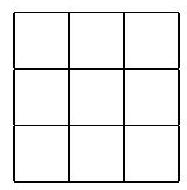
\includegraphics[max width=\textwidth, center]{2024_11_21_1e8c4b47eb64ad7d9f09g-1}


\end{document}